\chapter{Theorie}\label{ch:data}

\section{Grafische Benutzeroberfläche}
Der Begriff Benutzerschnittstelle bezeichnet alle Komponenten eines interaktiven Systems, die dem Benutzer Interaktionsmöglichkeiten mit selbigem System bieten, um ein verfolgtes Ziel zu erreichen.
Die grafische Benutzeroberfläche (GUI) bezeichnet hierbei den sichtbaren Anteil des Systems und damit nur einen Teil der gesamten Benutzerschnittstelle, zu der auch nicht sichtbare Teile wie z.B. die Funktionslogik gehören\cite{Sarodnick.2016}.
Heutzutage sind die meisten Benutzeroberflächen auch grafische Benutzeroberflächen, mit denen in den häufigsten Fällen die Interaktion mit dem Nutzer über direkte Manipulation stattfindet\cite{Nielsen.1995?}.

\section{Ergonomie}
Unter Ergonomie versteht man im Allgemeinen die "Lehre von der menschlichen Arbeit und die Erkenntnis ihrer Gesetzmäßigkeiten"\cite{https:www.facebook.comArbeitsplatzergonomie.2014}.
Hierbei ist es wichtig zu verstehen, dass dabei der Fokus nicht ausschließlich auf einer technischen Komponente liegt, sondern das Zusammenspiel von Mensch, der zugeteilten Aufgabe und den verfügbaren Werkzeugen betrachtet wird\cite{Sarodnick.2016}.
In Bezug auf Software bedeutet Ergonomie also konkret diese gut handhabbar und benutzerorientiert zu gestalten.

\section{Usability}
Mit immer höherer Komplexität von Systemen und Anwendungen kam der Begriff und das Verlangen nach  "Benutzerfreundlichkeit"\ auf.
Dieser Begriff suggeriert das lediglich die einfache Benutzung eines Systems ausschlaggebend ist, vernachlässigt hierbei jedoch die Notwendigkeit den Nutzer beim Erreichen seiner Ziele passend zu unterstützen.
Dies ist auch der Grund dafür das bald, statt auf "Benutzerfreundlichkeit"\ auf "Gebrauchstauglichkeit" (engl. Usability) geachtet wurde.
Im Gegensatz zur Ergonomie handelt es sich bei Usability nicht um eine eigenständige wissenschaftliche Disziplin, sondern um eine qualitative Anforderung an ein System\cite{Sarodnick.2016}.
Konkret spricht man bei einer Software-Anwendung von einer hohen Usability, wenn sie von der für sie bestimmten Zielgruppe effizient verwendet werden kann, also das verfolgte Ziel zufriedenstellend erreicht wird\cite{Richter.2016}.
Hierfür ist es entscheidend sich bewusst zu machen, dass ein technisches System oder Software immer Teil eines großen Handlungsablaufes ist und dazu dient Schritte dieses Handlungsablaufes zu erledigen.
Deshalb muss das System den Anforderungen dieses Ablaufes entsprechen und darf während der Entwicklung nicht getrennt davon betrachtet werden\cite{Sarodnick.2016}.

Usability wird üblicherweise dadurch gemessen, indem man Nutzern, die der Zielgruppe entsprechen einige vordefinierte Aufgaben mit dem zu messenden System abschließen lässt. 
In einigen Fällen kann es allerdings auch unnötig sein eine Aufgabe vorzudefinieren, da die Messung auch im alltäglichen Arbeitsablauf mit dem System stattfinden kann.
In beiden Fällen ist es jedoch wichtig die Ergebnisse immer im Kontext des Nutzers und der absolvierten Aufgabe zu betrachten\cite{Nielsen.1995?}. 
Wie bereits erwähnt misst die Usability wie zufriedenstellend ein Ziel erreicht werden kann.
Deshalb ist es nicht möglich die Usability für ein komplette System zu messen, da diese immer Kontextabhängig ist, woraus sich auch die Notwendigkeit ergibt bei einer Usability Studie die Testpersonen identische, oder zumindest ähnliche Aufgaben ausführen zu lassen.
Ein Textprogramm kann beispielsweise gut geeignet sein, um einen Brief zu tippen, jedoch völlig ungeeignet um größere Datenmengen zu verwalten. Es würde also für die eine Aufgabenstellung eine hohe Usability und für die andere eine niedrige aufweisen. 
Würde man diese Ergebnisse kontextunabhängig vergleichen würde keine valide Aussage über die Usability des Systems getroffen werden.

Für gewöhnliche ist Usability an fünf Attributen gut messbar, welche im Folgenden deshalb kurz erläutert werden.

\paragraph{Erlernbarkeit}
Das Attribut der Erlernbarkeit ist in vielerlei Hinsicht das fundamentalste von allen hier aufgeführten, da die erste Interaktion, die ein Nutzer mit einem System hat meist das erlernen dessen Funktionen beinhaltet.
Gemessen wird dieses Attribut ganz simpel mithilfe von Nutzern, indem man die Zeit misst, die diese benötigen um ein vorher festgelegtes Level an Kompetenz zu erreichen.
Um einzustufen ob dieses Level erreicht wurde kann beispielsweise überprüft werden ob der Nutzer eine bestimmte Aufgabe ohne Probleme, oder in einem gesetzten Zeitlimit bewältigen kann.
Die Testpersonen sollten der letztendlichen Zielgruppe entsprechen und das System vorher noch nicht genutzt haben\cite{Nielsen.1995?}.

\paragraph{Effizienz}
Sobald die Lernkurve des Nutzers nicht mehr rapide ansteigt, wie es bei der anfänglichen Nutzung eines Systems meist der Fall ist, fokussiert er sich darauf effizient  und produktiv mit dem System arbeiten zu können.
Da effizientes arbeiten nur ab einem gewissen Wissensgrad möglich ist, sollte bei der Messung dieses Attributes auf Testpersonen zurückgegriffen werden die bereits Erfahrung mit dem System haben, gegebenenfalls sogar Experten sind.
Die Einstufung, ab wann ein Nutzer als Experte gilt, kann entweder der Nutzer selbst treffen, oder man setzt voraus das Personen nach einem festgelegtem Benutzungszeitraum als Experten gelten.
Eine typische Art um Effizienz zu messen ist es, mit einer der genannten Möglichkeiten einen Nutzer als Experte einzustufen, Testpersonen zu finden die diesen Kriterien entsprechen und die Zeit zu messen die diese Personen benötigen um Testaufgaben abzuschließen\cite{Nielsen.1995?}.

\paragraph{Wiedererkennungswert}
Neben Experten und neuen Nutzern gibt es noch die Gruppe der gelegentlichen Nutzer eines Systems.
Für diese Gruppe ist das Attribut der Wiedererkennung besonders wichtig, da sie im Gegensatz zu neuen Nutzern nicht lernen müssen wie das Programm funktioniert, sondern sich lediglich an bereits Erlerntes erinnern müssen.
Das Attribut der Erlernbarkeit wirkt also ebenfalls unterstützend um einem System einen hohen Wiedererkennungswert zu geben, aber prinzipiell gilt es zu beachten das das neu Erlernen eines Systems eben nicht mit dem Wiedereinstieg in selbiges gleichzusetzen ist.
Diese beiden Attribute können sich also durchaus gegenseitig unterstützen, sind jedoch nicht austauschbar.
Messbar ist der Wiedererkennungswert prinzipiell durch zwei Methoden.
Eine davon ist die Durchführung eines Standard Tests mit Nutzern die einige Zeit nicht mit dem System interagiert haben durchzuführen und die Zeit zu messen die sie benötigen um spezifizierte Aufgaben abzuschließen.
Alternativ kann man einen Test durchführen bei dem die Erinnerungen der Testpersonen geprüft werden.
Hierbei werden die Nutzer nach dem Test gebeten die Effekte verschiedener Interaktionen, das Aussehen von Icons und die Bezeichnung bestimmter Befehle zu benennen.
Die Anzahl der korrekten Antworten die man hierbei erhält legt den Wiedererkennungswert des Systems fest.
Obwohl diese zweite Testvariante leichter durchzuführen ist, hat sie die Schwäche, vor allem bei komplexeren Systemen, nicht sonderlich aussagekräftig zu sein.
Es wurde festgestellt das Nutzer sich hier nicht an genaue Bezeichnungen oder Aussehen der Befehle erinnern konnten, jedoch kein Problem hatten diese in den Arbeitsabläufen zu finden oder zu nutzen.
Deshalb ist der erste Testansatz empfehlenswerter, auch wenn dieser mehr Aufwand mit sich bringt\cite{Nielsen.1995?}.

\paragraph{Fehler}
Nutzer sollten während ihrer Interaktion mit dem System so wenig Fehler wie möglich machen. 
Unter einem Fehler versteht man in diesem Zusammenhang jede ausgeführte Aktion durch die nicht das gewünschte Ergebnis erzielt wird.
Die Fehlerrate eines Systems wird dementsprechend daran gemessen wie viele Fehler einem Nutzer unterlaufen während er eine Aufgabenstellung bearbeitet, und kann deshalb begleitend zu anderen Attributen untersucht werden\cite{Nielsen.1995?}.

\paragraph{Zufriedenheit}
Das letzte Attribut der Usability ist die Zufriedenheit, welche sich in diesem Fall darauf bezieht wie angenehm es für den Nutzer ist mit einem System zu interagieren.
Zum einen kann dieses Attribut medizinisch, zum Beispiel mit Hilfe von EEGs, der Beobachtung der Pupillenerweiterung oder der Herzrate untersucht werden.
Da die Testpersonen jedoch meist ohnehin aufgeregt sind, sind solche zusätzlichen medizinischen Maßnahmen einer gewünschten entspannten Atmosphäre nicht zuträglich, abgesehen davon das der Aufwand für solche Untersuchten sehr hoch ist.
Eine andere Methode die Zufriedenheit zu messen, ist es, die Nutzer einfach direkt zu fragen.
Da man eine objektive Einschätzung der Zufriedenheit der Nutzer erhalten will ist es hier natürlich nötig mehrere Nutzer zu befragen, um aus den einzelnen subjektiven Meinungen eine objektive Meinung zu erhalten\cite{Nielsen.1995?}.
Diese Befragung findet meist in Form eines Fragebogens statt, da diese recht komplexe Art der Evaluierung in dieser Arbeit jedoch keine Verwendung findet, werden die Vorgehensweisen an dieser Stelle nicht weiter erläutert.

Da es sich bei der in dieser Arbeit untersuchten Software EB Guide Studio, näherer hierzu in Abschnitt 2.8, um eine Anwendung handelt mit der die meisten Nutzer über einen längeren Zeitraum auf hohem Niveau arbeiten, wird in dieser Usabilitystudie hauptsächlich das Attribut der Effizienz untersucht. Ergänzend dazu wird noch dokumentiert wie viele Fehler bei dem Nutzer durch die neuen Ergänzungen im Interface entstehen. Genaueres zu den Untersuchungen und Messungen folgt in Kapitel 5 dieser Arbeit.

\section{User Experience}
Entgegen einer häufigen Annahme bezeichnen Usability und User Experience (UX) nicht das Gleiche.
Usability bezeichnet lediglich ein Teil der gesamten User Experience eines Systems\cite{Knight.2019c}.
UX bezieht sich nicht nur auf die reine Nutzungszeit eines Systems, sondern berücksichtigt auch den Zeitraum davor und danach, bezeichnet als Antizipierte Nutzung und Verarbeitung der Nutzungssituation.
Usability ist hierbei, wie in \cref{fig:UX} zu sehen, als wichtiger Faktor der User Experience in der aktiven Nutzungsphase zu betrachten, jedoch nicht mit dem Begriff gleichzusetzen \cite{Sarodnick.2016}.
Durch die zusätzliche Betrachtung der Effekte auf den Nutzer vor und nach der Nutzung, wie beispielsweise Erwartungen an das Produkt und Akzeptanz des selbigen, entstehen hier auch Verbindungen zur Gestaltung der Benutzerschnittstelle und dem Produkt-Design\cite{Richter.2016}.
Zusammenfassend lässt sich festhalten das Usability zwar die funktionsbezogene Betrachtungsweise abdeckt, die User Experience als Ganzes jedoch auch emotionale Faktoren bezüglich des Designs und der Ästhetik berücksichtigt um das Nutzungsvergnügen möglichst hoch zu halten.
Zusätzlich ist eine gute User Experience notwendig, wenn ein Produkt auf dem Markt bestehen will.
Sobald es mehr als ein Produkt zur Lösung der gleichen Aufgabenstellung gibt, wird das mit der besseren User Experience Verwendung finden\cite{Knight.2019c}.


\begin{figure}[H]
\begin{center}
  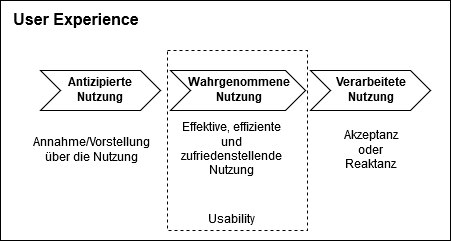
\includegraphics[scale=0.6]{figures/UX.png}
  \caption{Zusammenhang Usability und User Experience (nach \cite{Sarodnick.2016})}
  \label{fig:UX}
\end{center}
\end{figure}

\section{Kognitive Last}
Die Kognitive Last – auch als mentale Auslastung bekannt – bezeichnet im Allgemeinen die Differenz zwischen den Ressourcen (kognitiv, psychomotorisch oder wahrnehmend) die benötigt werden, um eine Aufgabe zu erfüllen, und den tatsächlich zur Verfügung stehenden Ressourcen. Die Größe der kognitiven Last beeinflusst also direkt die Leistung, die wir bei der Ausführung einer bestimmten Aufgabe erbringen können. Bei einer optimalen Auslastung erbringen Menschen maximale Leistung, ist sie hingegen zu klein oder zu groß geht die Leistung zurück, was in einem Fall auf Unterforderung und damit einhergehende Langweile, im anderen Fall auf Überlastung und Ablenkung zurückzuführen ist\cite{.e}. Beim Führen eines Fahrzeuges ist die Leistung des Fahrers beispielsweise maximal, wenn seine gesamte Aufmerksamkeit dem Fahren gilt. Allerdings wird er durch Nebentätigkeiten, wie zum Beispiel das Reagieren auf Warnungen, dazu gezwungen sein Multitasking zu betreiben, was seine Performance in Bezug auf beide Tätigkeiten einschränken wird. Es ist also auch wichtig abzuwägen, wie man Warnungen in Benutzeroberflächen darstellt, um keine mentale Überlastung des Benutzers hervorzurufen. Beim Fahren ist beispielsweise die visuelle Modalität durch den ständigen Blick auf die Straße schon sehr ausgelastet, weshalb zur Darstellung von Warnung auch aus Gründen der Auslastung auf Warnungen in Form von Videos oder Animationen verzichtet werden sollte und eher auf die anderen, bereits aufgeführten Modalitäten des Menschen ausgelagert werden sollte.

\section{Human - centered  design process}
Human-centered design ist ein Ansatz zur Entwicklung interaktiver Systeme, welcher das Ziel verfolgt möglichst nützliche Systeme zu entwickeln und diese gut benutzbar zu machen.
Das wird vor allem durch das fokussieren auf den Benutzer und dessen Bedürfnisse und durch die Anwendung von Ergonomie, Wissen und Techniken der Usability während des Entwicklungsprozesses erreicht\cite{.}.
Der in \cref{fig:HCD} zu sehende User Experience Engineering Process beschreibt den Human Centered Design Process für Elektrobit und basiert auf der ISO Norm 9241 - 210.
Das Model sieht Iterationen benutzerorientierter Aktivitäten vor, durch die fortlaufend der Erkenntnisstand der Entwickler erhöht wird, was bei dem ursprünglichen Ansatz eines Wasserfallmodells nicht der Fall war.

\begin{figure}[H]
\begin{center}
  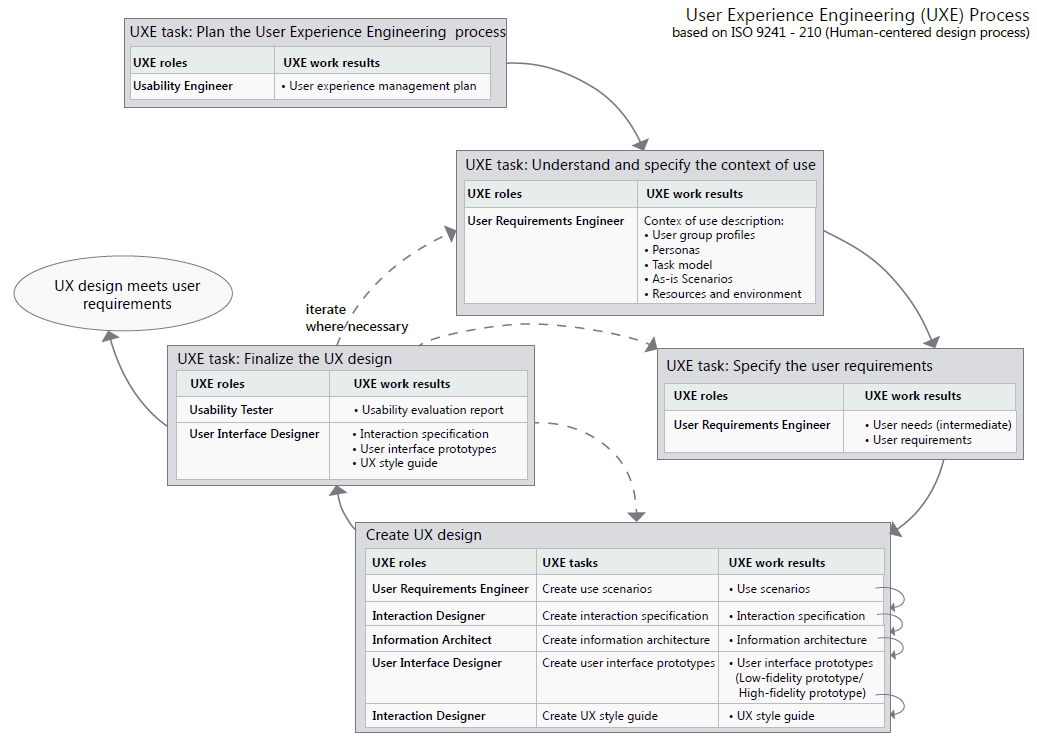
\includegraphics[width=\textwidth]{figures/HCD.png}
  \caption{Human - Centered - Design - Process bei Elektrobit}
  \label{fig:HCD}
\end{center}
\end{figure}

Die ISO 9241-210 Norm beschreibt das benutzerorientierte Vorgehen in Entwicklungsprojekten, und gibt Anregungen wie Usability-Engineering-Aktivitäten im Entwicklungsprojekt angewendet werden können.
Allgemein definiert die Norm das Vorgehen so, dass die Gestaltung des Systems auf vorangehenden Analysen der Nutzer, deren Arbeitsaufgaben und Arbeitsabläufen aufbaut.
Um aussagekräftige Analysen zu erhalten werden die Nutzer während des Entwicklungsprozessen immer wieder aktiv mit einbezogen, was vor allem durch die fest eingeplanten Iterationen geschieht.
Optimalerweise vereint das Gestaltungsteam fachübergreifende Kenntnisse und kann die in \cref{fig:HCD} benannten Rollen optimale besetzen\cite{.d}.

Der Human-centered design process kann und sollte bei der Entwicklung jedes interaktiven Systems verwendet werden, welches eine Benutzeroberfläche aufweist, und wird deshalb auch in der Entwicklung dieser Bachelorarbeit angewendet werden.
Aufgrund der Tatsachen, dass bei dieser Arbeit einerseits eine zeitliche Einschränkung vorliegt, und andererseits die Bearbeitung von einer Person und nicht von einem Team durchgeführt wird werden die Iterationen und die einzelnen Schritte jedoch in einer abgeschwächten Form durchgeführt werden. Genauerer Erläuterungen dazu finden sich in den entsprechenden Abschnitten dieser Arbeit.

\section{Gestaltprinzipien der Usability}
Durch die Interaktion mit einem Produkt oder einer Anwendung entstehen bei Nutzern immer Erfahrungen.
Ob diese Erfahrungen positiv oder negativ behaftet sind wird maßgeblich dadurch beeinflusst ob das Design der Anwendung den Nutzer unterstützt oder eher behindert, also ob die User Experience gut oder schlecht ist.
Bei der Interaktion mit einem Produkt muss der Nutzer immer herausfinden wie er mit ihm umgehen soll, welche Funktionen es bietet oder was überhaupt der Sinn des Produktes ist.
Diese Eigenschaft wird als Discoverability oder Erkennbarkeit bezeichnet und ist für eine gute User Experience möglichst hoch zu halten.
Discoverability resultiert aus denen im  Folgenden erläuterten Gestaltprinzipien der Usability, weshalb diese bei jeden Entwurf eines Systems berücksichtigt und einbezogen werden sollten\cite{Norman.2016}.

\subsection*{Konsistenz}
Konsistenz im Design wirkt sich insofern positiv auf die Usability eines Systems aus, das die Benutzbarkeit steigt, wenn gleiche Funktionen in einem System auch auf identische Art und Weise dargestellt werden.
Dadurch wird es dem Nutzer ermöglicht bereits Gelerntes in einem neuen Kontext anzuwenden, ohne effektiv darüber nachdenken zu müssen, neue Dinge schneller zu lernen und sich auf die relevanten Dinge einer Aufgabe zu konzentrieren.
Konsistenz in Systemen lässt sich in vier Kategorien unterteilen, die im Folgenden jeweils kurz erläutert werden.

\paragraph{Ästhetische Konsistenz}
Ästhetische Konsistenz bezieht sich auf Konsistenz in Stil und Aussehen. Dadurch entsteht ein hoher Wiedererkennungswert und es wird Zugehörigkeit signalisiert. Das einfachste Beispiel hierfür ist ein Firmenlogo, welches immer mit konsistenter Schriftart und Farbgebung auftaucht.

\paragraph{Funktionale Konsistenz}
Funktionale Konsistenz bezieht sich auf die Konsistenz von Bedeutung und Aktion, beispielsweise zeigt eine Ampel immer orange bevor sie rot wird. Der Nutzer kann also sicher mit einer immer gleichen darauffolgenden Aktion auf den aktuellen Zustand rechnen. 
Usability und Lernfähigkeit werden durch funktionale Konsistenz erhöht, indem diese bereits verinnerlichten Abläufe einfach auf neue Situationen übertragen werden können. So wird beispielsweise ein einheitlicher Playbutton für alle Geräte, von Kassettenrekorder bis Streamingdienst, verwendet.
Die Nutzung bereits bekannter Symbole ermöglicht dem Nutzer also eine intuitive Interaktion und macht es möglich die Aufmerksamkeit auf unbekannte Aspekte zu richten, die tatsächlich noch neu gelernt werden müssen.

\paragraph{Interne Konsistenz}
Interne Konsistenz bezieht sich auf Konsistenz mit anderen Elementen im System, beispielsweise sind Wegweiser in einem Park konsistent zueinander.
Dies erzeugt ein Vertrauensgefühl bei den Nutzern, und vermittelt ein durchdachtes Designkonzept und erweckt nicht den Eindruck das alle Komponenten einfach zusammengewürfelt wurden.

\paragraph{Externe Konsistenz}
Externe Konsistenz bezieht sich auf Konsistenz mit anderen Elementen in der Umgebung. Die Vorteile der internen Konsistenz werden hierbei systemübergreifend erweitert. Das Erreichen externer Konsistenz gestaltet sich jedoch auch schwieriger, da unabhängige Systeme selten exakt gleiche Designstandards haben.

Nicht alle dieser Konsistenzstandards können oder sollten in allen Fällen angewendet werden. 
Es lässt sich jedoch festhalten das Elemente in einer logischen Gruppe immer ästhetisch und funktional konsistent sein sollten.
Insgesamt sollte ästhetische und funktionale Konsistenz, wann immer möglich berücksichtigt werden, da durch ästhetische Konsistenz bei der Einführung einmaliger Identitäten Wiedererkennung gewährleistet werden kann und funktionale Konsistenz aus den bereits genannten Gründen die Usability eines Systems erhöht.
Abschließend sollten Systeme immer eine interne Konsistenz aufweisen, sollten bereits Designstandards existieren, gilt es diese zu analysieren.\cite{Lidwell.2010}

\subsection*{Sichtbarkeit}

Das Prinzip der Sichtbarkeit besagt, dass Systeme benutzbarer sind, wenn der aktuelle Status des Systems, mögliche Aktionen und deren Auswirkungen für den Nutzer deutlich erkennbar sind.
Es beruht auf der Erkenntnis, dass Menschen schneller und besser Lösungswege finden wenn sie aus einer Reihe von Optionen auswählen können, anstatt sich selbstständig an alle Möglichkeiten aus dem Stegreif erinnern zu müssen\cite{Lidwell.2010}.
Das macht es zu dem wichtigsten Prinzip für hohe Usability in komplexen Systemen, jedoch auch zu dem, welches am meisten verletzt wird\cite{Norman.2016}.
Häufig wird versucht alle möglichen Optionen, die ein System bietet sichtbar zu machen, was vor allem in komplexeren Systemen dazu führt das sie relevanten Optionen durch Informationsüberladung auf Seiten des Nutzers schwerer zu erreichen sind. 
Anstatt die Usabilty zu erhöhen wird also genau das Gegenteil erzielt.
Lösungen für diese Problemstellung sind beispielsweise eine Hierarchische Anordnung der Elemente oder Kontextsensitivität des Systems.
Bei der Hierarchischen Anordnung werden Funktionen und Informationen in logische Kategorien unterteilt und in übergeordneten Menüs versteckt, welche bei Bedarf ausgeklappt werden können. Ein Beispiel hierfür ist ein Dropdownmenü, wie man es von vielen Websites kennt.
In einem Kontextsensitiven System werden Aktionsmöglichkeiten und Informationen je nach aktuellem Status des Systems versteckt oder angezeigt. Beispielsweise bekommt man in einer Modellierungssoftware mit unterschiedlichen Elementen immer nur die Properties angezeigt die für das aktuell ausgewählte Element relevant sind, und nicht alle Properties die im gesamten System existieren\cite{Lidwell.2010}.


\subsection*{Affordanz}

Affordanz bezeichnet die Möglichkeiten mit einem Objekt zu interagieren. Beispielsweise kann eine Checkbox an und wieder abgewählt oder ein Schieberegler nach oben und unten geschoben werden.
Die sichtbare Affordanz bezeichnet die Eigenschaft das einem Objekt die Interaktionsmöglichkeiten bereits angesehen werden können, ohne mit ihm interagiert zu haben.
Sichtbare Affordanz ist vor allem in der User Interface Gestaltung wichtig, weil praktisch betrachtet alle Pixel auf einem Bildschirm anklickbar sind, jedoch in den meisten Fällen keine Aktion durch das klicken ausgelöst wird.
Deshalb ist es wichtig dem Nutzer durch das Aussehen der Elemente zu vermitteln ob diese, wenn sie geklickt werden eine Aktion auslösen, um dem Nutzer wahlloses Klicken durch das Interface zu ersparen, bis ein interaktives Objekt gefunden wird.
Solche Probleme können visuell gelöst werden, indem man Objekte im User Interface wie Objekte in der echten Welt aussehen lässt, also beispielsweise einen Button dreidimensional gestaltet.
Alternativ kann man beispielsweise alle anklickbaren Objekte etwas anders gestalten als den Rest der Objekte im Interface, um dem Nutzer zu vermitteln das hier eine Interaktion stattfinden kann\cite{Knight.2019c}.

\subsection*{Rückmeldung}

Eine der grundlegendsten Richtlinien um die Usability eines Systems zu erhöhen, ist es dem Nutzer immer eine Rückmeldung auf seine Aktionen zu geben.
Das bedeutet dem Nutzer immer den aktuellen Systemstatus anzuzeigen und wie seine Aktion vom System interpretiert wurde.
Eine Rückmeldung ist vor allem auch dann wichtig, wenn die gewünschte Aktion nicht erfolgreich vom System ausgeführt wurde
Durch fehlende Rückmeldungen kommt Misstrauen beim Nutzer auf, weil ihm nicht vermittelt wird ob auf seine Aktionen auch eine Reaktion des Systems erfolgt\cite{Knight.2019c}.
Dieses Problem tritt beispielsweise auf, wenn ein System lange braucht um eine Eingabe zu verarbeiten und es versäumt dies dem Nutzer mitzuteilen.
So ein Verhalten könnte zur fälschlichen Annahme führen das System wäre kaputt, oder dazu das der Nutzer beginnt neue Interaktionsmöglichkeiten anzuklicken.
Reagiert das System innerhalb 0.1 Sekunden, nimmt der Nutzer dies als sofortiges Feedback wahr und keine gesonderte Meldung ist nötig.
Bewegt sich die Reaktionszeit zwischen 0.1 und 1.0 Sekunden ist für gewöhnlich auch keine besondere Rückmeldung vom System nötig, auch wenn der Nutzer hier bereits nicht mehr das Gefühl hat direkt mit den Daten zu interagieren, da eine kurze Verzögerung stattfindet.
Sobald die Wartezeit auf Seiten des Nutzers jedoch eine Sekunde überschreitet sollte sich der Cursor in eine Sanduhr oder ähnliches verwandeln und damit die Rückmeldung geben, dass das System beschäftigt ist.
Sollte die systemseitige Verarbeitung der Eingabe länger als 10 Sekunden dauern ist es ratsam die Ladeanzeige durch eine konkrete Fortschrittsleiste zu ersetzen\cite{Nielsen.1995?}.

\subsection*{Mapping}
Mapping bezeichnet die Beziehung zwischen Bedienelementen und den Effekten den deren Aktivierung auslöst.
Wenn der Effekt den eine Nutzerinteraktion nach sich zieht, den Erwartungen des Nutzers entspricht, handelt es sich um gutes Mapping.
Die ist beispielsweise bei einem elektronischen Fensterheber der Fall. Wird hier der Hebel nach oben bewegt, hebt sich das Fenster, bewegt man den Hebel nach unten senkt es sich.
Gutes Mapping wird zum Großteil durch Ähnlichkeit, das Verhalten oder der Bedeutung innerhalb eines Layouts erreicht.
Entspricht beispielsweise das Layout von Herdplattenreglern der Anordnung der Platten wird gutes Mapping durch das Layout erzeugt, der bereits beschriebene Fensterheber arbeitet mit dem Verhalten, und die Tatsache das ein Notfallknopf rot eingefärbt wird ist darauf zurückzuführen das die meisten Menschen rot mit Gefahr oder dem Stopplicht einer Ampel assoziieren.
In jedem dieser Fälle macht die Ähnlichkeit es möglich den Effekt der Handlung vorherzusehen, und vereinfacht dadurch die Bedienung für den Nutzer.
Aktionsmöglichkeiten müssen so platziert werden das ihre Position und ihr Verhalten dem Layout und dem Verhalten die Anwendung angepasst sind. 
Außerdem sollte es vermieden werden durch eine identische Aktion verschiedene Reaktionen auszulösen\cite{Lidwell.2010}.

\subsection*{Einschränkungen}
Einschränkungen in einem System limitieren die Interaktionsmöglichkeiten für den Nutzer.
Wird beispielsweise ein Button ausgegraut, der im aktuellen Kontext ohnehin keine Aktion ausführen würde wird der Nutzer rein optisch daran gehindert eine nicht zielführende Aktion auszuführen.
Durchdachte Einschränkungen dieser Art machen ein Design einfacher nutzbar und reduziert deutlich die Wahrscheinlichkeit von Fehlschlägen während der Systeminteraktion \cite{Lidwell.2010}.


\paragraph{Physische Einschränkungen}
Physische Einschränkungen limitieren den Bereich in den Aktionen ausgeführt werden können, indem sie Eingaben des Nutzers umwandeln oder umleiten.
Eine Art der Einschränkungen ist das konvertieren der Eingabe in lineare oder kurvenförmige Bewegung, wie es Beispielsweise bei der Interaktion mit einer Scrollbar der Fall ist.
Mithilfe von Achsen können wirkende Kräfte in Rotationsbewegungen umgewandelt werden, was eine Kontrolloberfläche mit unendlicher Größe auf einem kleinen Feld erzeugt, was am Beispiel der Computermaus gut zu erkennen ist.
Die Letzte Form der Einschränkung passiert über Barrieren, die die Eingabe verlangsamen, komplett ausbremsen oder umleiten. Die Einfassung eines Computerbildschirms beschränkt beispielsweise physisch die Interaktionsfläche für den Nutzer.
Allgemein sind Physische Einschränkungen nützlich um die Anzahl fehlerhafter Eingaben zu vermeiden, oder manche Eingaben erst gar nicht zu ermöglichen\cite{Norman.2016}.

\paragraph{Psychologische Einschränkungen}
Psychologische Einschränkungen limitieren die Anzahl möglicher Aktionen durch Nutzung des Wissens über das Verhalten und die Denkweise der Nutzer.
Dies passiert durch den Einsatz von Symbolen, nutzen bekannter Konventionen oder durch das bereits erwähnte Mapping.
Symbole sind sinnvoll um Dinge zu benennen, zu erklären oder auch um Warnungen visuell, auditiv oder fühlbar darzustellen.
Mit Konventionen macht man sich bekannte Interaktionsmöglichkeiten zunutze, weshalb sie sich gut eignen Systeme sowohl konsistent als auch leicht benutzbar zu machen.
Mappings sind, aus bereits erwähnten Gründen, nützliche um dem Benutzer zu vermitteln welche Aktionen aufgrund der Sichtbarkeit, Position oder dem Aussehen der Elemente möglich sind\cite{Norman.2016}.

Zusammenfassend sollten Einschränkungen im Allgemeinen verwendet werden um die Benutzbarkeit eines Systems zu vereinfachen und die Anzahl an Fehlern zu minimieren. Physische Einschränkungen dienen hierbei eher dem Verhindern ungewollter Eingaben oder gefährlicher Aktionen, Psychologische Einschränkungen sollen das Design eines Systems für den Nutzer klarer und intuitiver gestalten.

\subsection*{Vorteile für den Nutzer}
Durch das Befolgen der soeben erläuterten Gestaltprinzipien bei dem Entwurf eines User Interfaces, ist es möglich sich die Art und Weise wie Nutzer visuelle Reize verarbeiten zunutze zu machen um die Benutzerfreundlichkeit des Systems zu erhöhen.
Das passiert vor allem dadurch, dass man die kognitive Last des Nutzers verringern während er sich mit dem Interface auseinandersetzt, indem man bereits bekannten Gestaltprinzipien nutzt.
Das bedeutet, dass der Nutzer seine Energie nicht darauf verschwenden muss darüber nachzudenken wie mit den Bestandteilen des Interfaces interagiert werden kann, oder was deren Funktionen sein könnten\cite{Knight.2019c}.

\section{EB Guide Studio}
Wie bereits in Abschnitt 1.2 erwähnt dient EB GUIDE der Entwicklung multimodalder HMIs.
Um nicht nur das Design sondern auch das Verhalten von User Interfaces bestimmen zu können und eine Auslieferung auf das Zielsystem zu ermöglichen besteht die Produktlinie EB GUIDE aus den verschiedenen, in \cref{fig:guide_puzzle} zu sehenden, Komponenten.
Hierbei wird zwischen Komponenten für das Graphical User Interface (GUI) und Komponenten für die Sprachsteuerung unterschieden.
Da die Sprachkomponenten jedoch für diese Arbeit nicht weiter relevant sind werden diese in den folgenden Kapiteln auch nicht genauer erläutert.
Innerhalb des GUI Bereiches bildet EB GUIDE Studio das tatsächliche Modellierungstool, mit dem das Verhalten und Aussehen der Benutzeroberfläche definiert wird.
Für das entwickelte Modell stellt das EB GUIDE Target Framework auf dem Zielsystem die Laufzeitumgebung bereit.\cite{.c}

\begin{figure} [H]
\begin{center}
  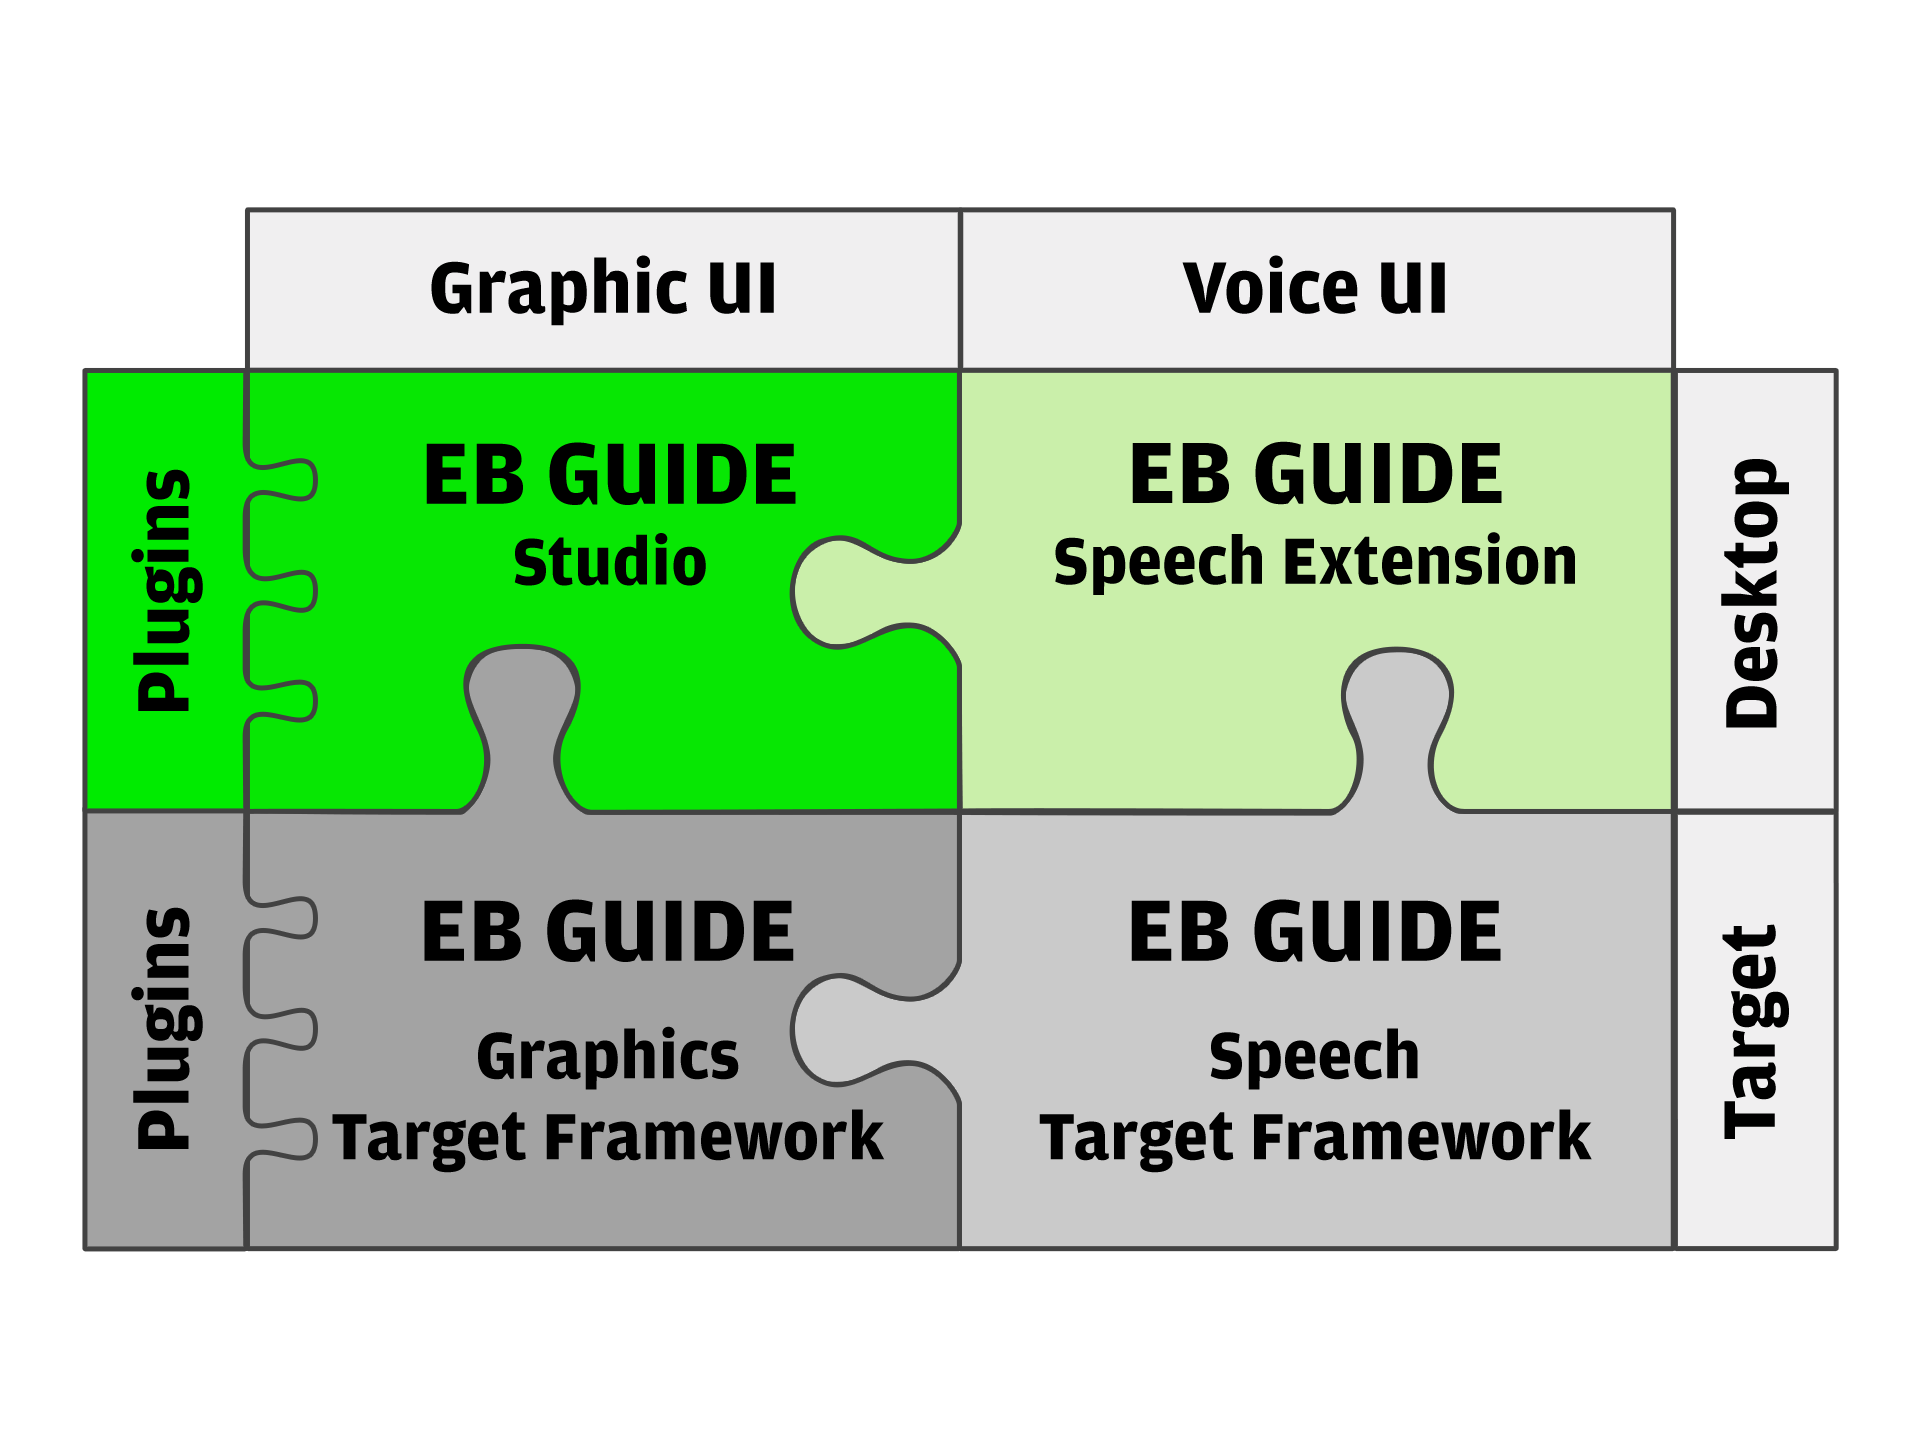
\includegraphics[scale=0.7]{figures/EB_GUIDE_Puzzle.png}
  \caption{Aufbau EB GUIDE}
  \label{fig:guide_puzzle}
\end{center}
\end{figure}

EB Guide Studio ist das Interface von EB Guide mit dem nach dem What-You-See-Is-What-You-Get (WYSIWYG) Prinzip User Interfaces modelliert werden. 
Durch das WYSIWYG Prinzip ist es während des Modellierens einer View bereits möglich das Endergebnis des Designs zu sehen.
Das Verhalten des Interfaces hingegen wird mithilfe einer Zustandsmaschine, der sogenannten Statemachine, modelliert die auf dem UML- Prinzip aufbaut.
Die Trennung der Logik und des Designs wird in EB GUIDE Studio grafisch durch zwei unterschiedliche Arbeitsoberflächen gestaltet in welchen den Modellierern jeweils die entsprechenden Tools und Elemente zur Verfügung stehen.

\begin{figure} [H]
\begin{center}
  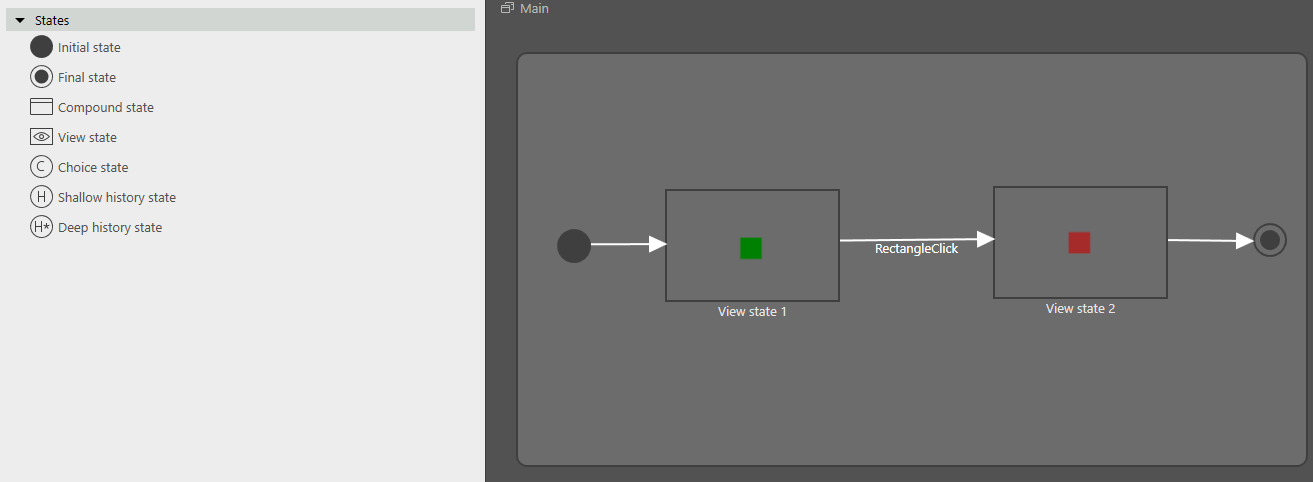
\includegraphics[scale=0.4]{figures/Guide_Statemachine.PNG}
  \caption{EB Guide Studio Statemachine}
  \label{fig:Guide_Statemachine}
\end{center}
\end{figure}

In \cref{fig:Guide_Statemachine} ist die Statemachine für ein simples Beispiel zu sehen.
Links neben der Arbeitsfläche befindet sich eine Toolbox mit deren Inhalt per Drag and Drop auf der Arbeitsfläche die benötigte Logik definiert wird.
Wie bei UML-Diagrammen gibt es einen Initial State der den Startpunkt angibt und einen Final State der die Statemachine beendet.
Die ebenfalls zu sehenden View States stehen für einen Screen im Endprodukt, dementsprechend wird in den View States auch das Aussehen der Interfaces definiert.
Die Verbindungen zwischen den States werden als Transitionen bezeichnet und mithilfe von Events ausgelöst.
Events stellen hierbei beliebige Ereignisse dar die durch Elemente in der View ausgelöst werden können.
Der Auslöser für das Event wird mithilfe einer eigens für EB Guide entwickelten Skriptsprache als Trigger für dieses gesetzt.
Die häufigsten Auslöser sind Benutzeraktionen mit Widgets, die in \cref{fig:Guide_View}zu sehen sind.
Widgets sind Elemente, mit denen das Aussehen des Interfaces im sogenannten View Editor bestimmt wird und die sich in Basis- und 3D-Widgets einteilen lassen.
Alle Basiswidgets verfügen über Basiseigenschaften wie Höhe, Breite und Farbe sowie über spezifische Eigenschaften wie zum Beispiel "Touch-Released" bei einem Button.\cite{studio_guide}
Beipspielsweise wird das Event "RectangleClick", was sich in \cref{fig:Guide_Statemachine} an der Transition zwischen View State 1 und View State 2 befindet in diesem Beispiel durch das Klicken auf das grüne Rechteck in View State 1 ausgelöst.
Ist die Benutzeraktion abgeschlossen findet der Übergang von View State1 zu View State 2 statt und der Nutzer sieht nun anstatt dem grünen ein rotes Rechteck.
Damit diese Aktion erfolgreich ausgeführt wird muss das grüne Rechteck die Eigenschaft "Touch-Released"\ zugewiesen bekommen und über die EB Guide Skriptsprache mitgeteilt bekommen das Event RectangleClick zu feuern sobald das grüne Rechteck berührt wurde.
Da sich dieses Event in der Statemachine an der Transition zwischen den beiden States befindet wird nun durch einen Klick auf das grüne Rechteck ein Bildschirmwechsel zwischen den beiden View States ausgelöst.

\begin{figure}[H]
\begin{center}
  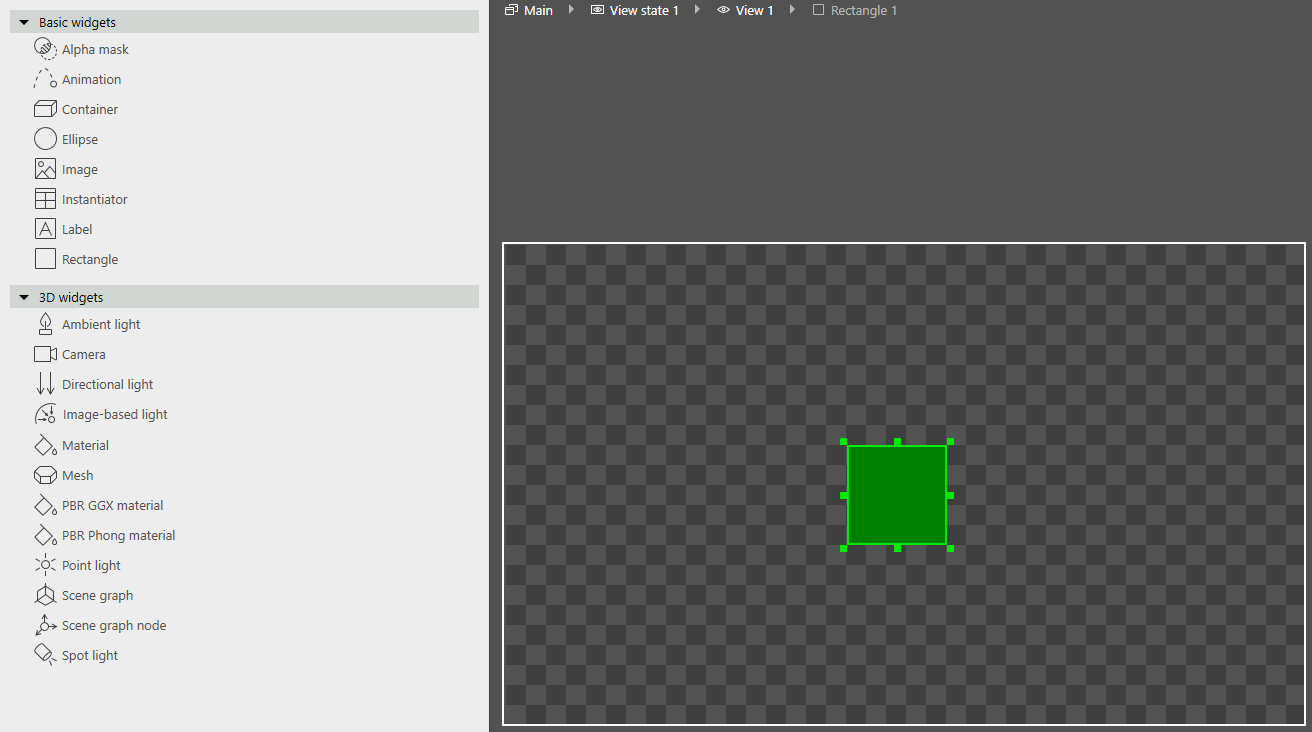
\includegraphics[scale=0.4]{figures/Guide_View.PNG}
  \caption{EB Guide VIEW}
  \label{fig:Guide_View}
\end{center}
\end{figure}


